\documentclass[11pt]{article}

\usepackage[margin=1in]{geometry}
\usepackage{amsmath,amssymb,mathtools}
\usepackage{booktabs}
\usepackage{graphicx}
\usepackage{microtype}
\usepackage{float}

\title{Study Report on Regret Matching and Counterfactual Regret Minimization}
\author{}
\date{\today}

\begin{document}

\maketitle

\begin{abstract}
This report summarizes my study of extensive-form games (EFGs), tree-form sequential decision processes (TFSDPs), regret matching (RM), and counterfactual regret minimization (CFR). I also report two small experiments: RM/RM+ on Rock-Paper-Scissors and CFR/CFR+ on Kuhn Poker. The main goal was not only to implement the algorithms, but also to clarify several notation and modeling details that were initially confusing when reading different sources.
\end{abstract}

\section{Introduction}

\subsection{EFGs and TFSDPs}

An extensive-form game (EFG) describes a sequential game as a tree. Histories correspond to nodes in the tree, terminal histories carry utilities, and each non-terminal history belongs either to chance or to one of the players. Information sets encode imperfect information: if two histories belong to the same information set of player $i$, then player $i$ cannot distinguish them when choosing an action. In two-player zero-sum games, the objective is to find a strategy profile close to a Nash equilibrium.

A TFSDP is a player-centric representation of sequential decision making. Instead of storing the full game tree at once, it describes a single player's local structure using observation points, decision points, signals, actions, and transition maps. In the implementation used for this project, a TFSDP is represented by
\[
(J, A, K, S, \rho, \Sigma, p),
\]
where $J$ is the set of decision points, $A_j$ is the action set at $j \in J$, $K$ is the set of observation points, $S_k$ is the signal set at $k \in K$, $\rho$ is the transition map, $\Sigma$ is the set of sequences, and $p_j$ denotes the parent sequence of decision point $j$. This is a convenient representation for sequence-form strategies and for implementing CFR as a collection of local regret minimizers.

One modeling detail that was initially confusing is that the same strategic game can have multiple equivalent EFG or TFSDP representations. For example, in Kuhn Poker the chance move that deals cards can be modeled either as two successive deals (first to player 1, then to player 2) or as a single chance node with six possible card pairs. These trees are not syntactically identical, but they represent the same strategic situation. This explains why different lecture notes or code bases sometimes present slightly different trees even when they are solving the same game.

\subsection{Regret Matching}

Regret Matching (RM) is one of the simplest no-regret procedures. Suppose a player repeatedly chooses a mixed action $x^t \in \Delta(A)$ and then observes a utility vector $\ell^t \in \mathbb{R}^{|A|}$. The cumulative regret for action $a$ after $T$ rounds is
\[
R^T(a) = \sum_{t=1}^{T} \left(\ell^t(a) - \langle x^t, \ell^t \rangle\right).
\]
RM chooses the next strategy by normalizing only the positive cumulative regrets:
\[
x^{T+1}(a) =
\begin{cases}
\dfrac{[R^T(a)]_+}{\sum_{b \in A} [R^T(b)]_+}, & \text{if } \sum_{b \in A} [R^T(b)]_+ > 0, \\[1.2ex]
\dfrac{1}{|A|}, & \text{otherwise},
\end{cases}
\]
where $[r]_+ = \max\{r, 0\}$.

The algorithm is remarkably simple: maintain cumulative regrets, keep only the positive part, normalize, and repeat. Regret Matching+ (RM+) modifies the update by truncating cumulative regrets at zero after every iteration. Although I omit the proof, the important practical point is that such a small change often improves convergence substantially.

\subsection{CFR and the Regret-Circuit Intuition}

Counterfactual Regret Minimization (CFR) extends the same idea to imperfect-information games. The original algorithm was introduced by Zinkevich et al.\ \cite{zinkevich2007}. Rather than minimizing regret over the entire normal-form strategy space directly, CFR decomposes the problem across information sets. Each information set is assigned a local regret minimizer, typically RM or RM+, and these local modules are wired together through the game tree.

This is exactly the viewpoint emphasized by regret circuits \cite{farina2019}. Each local module receives a linear utility vector computed from the rest of the tree, updates its own regrets, and outputs a behavioral strategy for that information set. The global strategy is then the composition of all these local decisions. Intuitively, CFR works because the counterfactual utility isolates the effect of a player's choice at a given information set while weighting the path to that information set only by the opponents' and chance's reach probabilities.

For player $i$, strategy profile $\sigma$, and information set $I$, the counterfactual value can be written as
\[
u_i(\sigma, I)
=
\frac{
\sum\limits_{h \in I}
\sum\limits_{z \in Z: h \sqsubset z}
\pi^\sigma_{-i}(h)\,\pi^\sigma(h, z)\,u_i(z)
}{
\pi^\sigma_{-i}(I)
}.
\]
The instantaneous counterfactual regret for action $a \in A(I)$ is the difference between the counterfactual value of deviating to $a$ at $I$ and the counterfactual value of following the current strategy at $I$. CFR accumulates these local regrets over time and applies regret matching independently at each information set. In two-player zero-sum games, the average strategy converges to equilibrium.

\subsection{A Notation Subtlety About Reach Probabilities}

One point that caused confusion while reading \cite{zinkevich2007} was the notation for the reach probability of an information set. The paper defines
\[
\pi^\sigma(I) = \sum_{h \in I} \pi^\sigma(h),
\]
and then states that $\pi_i^\sigma(I)$ and $\pi_{-i}^\sigma(I)$ are defined similarly. If one reads this too literally, it is tempting to write
\[
\pi_i^\sigma(I) = \sum_{h \in I} \pi_i^\sigma(h),
\]
but this is not the intended object.

For any information set $I$ of player $i$, perfect recall implies that $\pi_i^\sigma(h)$ is identical for every history $h \in I$. Therefore the natural interpretation is
\[
\pi_i^\sigma(I) = \pi_i^\sigma(h)
\qquad \text{for any } h \in I,
\]
while
\[
\pi_{-i}^\sigma(I) = \sum_{h \in I} \pi_{-i}^\sigma(h).
\]
With this interpretation,
\[
\pi^\sigma(I)
=
\sum_{h \in I} \pi_i^\sigma(h)\pi_{-i}^\sigma(h)
=
\pi_i^\sigma(I)\sum_{h \in I}\pi_{-i}^\sigma(h)
=
\pi_i^\sigma(I)\pi_{-i}^\sigma(I).
\]
This factorization is exactly what makes the counterfactual-value formula natural: the player's own reach to $I$ is constant across the histories in $I$, so it cancels, leaving only the opponents' and chance's contribution in the weighting. In hindsight the idea is simple, but it is easy to misread the notation when first encountering CFR.

\section{Experiments}

\subsection{Notebook 1: RM on Rock-Paper-Scissors}

The first experiment applies RM and RM+ to Rock-Paper-Scissors (RPS), a two-player zero-sum matrix game with a unique mixed Nash equilibrium at the uniform strategy. Since a uniform initial strategy is already an equilibrium, starting from zero regret would make the algorithm remain there immediately. To obtain a more informative learning curve, I initialized the cumulative regrets with non-uniform values and then ran self-play for $10{,}000$ iterations.

Exploitability was measured as $\text{NashConv}/2$. The final results were:
\begin{center}
\begin{tabular}{lccc}
\toprule
Algorithm & Player 0 average strategy & Player 1 average strategy & Final exploitability \\
\midrule
RM & $(0.3392, 0.3343, 0.3265)$ & $(0.3302, 0.3315, 0.3383)$ & $0.00977403$ \\
RM+ & $(0.3320, 0.3328, 0.3352)$ & $(0.3348, 0.3338, 0.3314)$ & $0.00287796$ \\
\bottomrule
\end{tabular}
\end{center}

Empirically, both methods showed a convergence trend roughly consistent with $O(1/T)$, and RM+ converged faster, as expected. However, an interesting feature of both curves is that they oscillate rather than decrease monotonically. My interpretation is that this is related to the rotational dynamics of RPS: instantaneous play naturally cycles around the mixed equilibrium, and averaging only partially smooths this effect. This suggests that purely first-order regret updates may be slowed down by cyclic behavior, and it would be interesting to compare them with more predictive or higher-order updates in the future.

\begin{figure}[H]
\centering
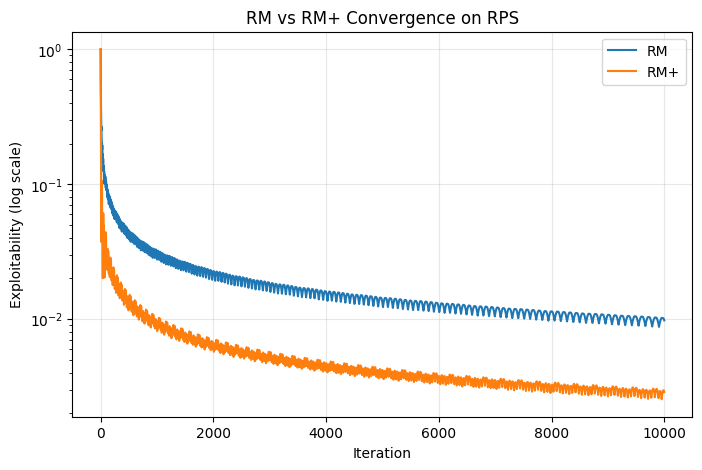
\includegraphics[width=0.82\linewidth]{figures/rps_rm_vs_rmplus.png}
\caption{Exploitability of the average strategy for RM and RM+ on Rock-Paper-Scissors.}
\label{fig:rps}
\end{figure}

\subsection{Notebook 2: CFR on Kuhn Poker}

The second experiment applies CFR and CFR+ to Kuhn Poker. In the implementation, the initial chance event is represented as a single node with six equally likely card deals. This choice is strategically equivalent to a deeper representation that deals cards one by one, but it is more compact and keeps the game tree easy to inspect.

Again I ran $10{,}000$ iterations and measured exploitability of the average strategy. The final results were:
\begin{center}
\begin{tabular}{lcc}
\toprule
Algorithm & Final value for Player 0 & Final exploitability \\
\midrule
CFR & $-0.055548$ & $0.00232917$ \\
CFR+ & $-0.055546$ & $0.00130270$ \\
\bottomrule
\end{tabular}
\end{center}

Both algorithms converged to strategies with very small exploitability, and CFR+ again converged faster than the vanilla version. The learned game value is also extremely close to the known value of Kuhn Poker, $-1/18 \approx -0.055556$, which provides a useful sanity check on the implementation. Qualitatively, the learned strategies also match the standard structure of the equilibrium: bluffing with the weakest card at a moderate frequency, betting aggressively with the strongest card, and mixing in the middle with the queen in response situations.

\begin{figure}[H]
\centering
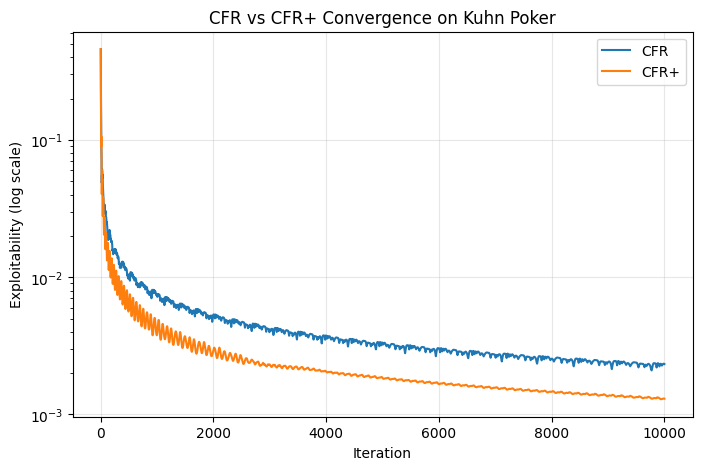
\includegraphics[width=0.82\linewidth]{figures/kuhn_cfr_vs_cfrplus.png}
\caption{Exploitability of the average strategy for CFR and CFR+ on Kuhn Poker.}
\label{fig:kuhn}
\end{figure}

\section{Conclusion}

This project helped clarify two complementary ideas. First, RM is an extremely simple regret minimizer, yet it already finds optimal mixed strategies in repeated zero-sum play. Second, CFR can be understood as wiring together many such local regret minimizers over an imperfect-information game tree. That viewpoint makes the algorithm feel much less mysterious than it first appears in the original paper.

The most useful conceptual takeaway for me was that both notation and representation matter. The same game may be written as different but equivalent EFGs or TFSDPs, and the notation for reach probabilities at an information set must be interpreted carefully. Once those points are clear, the overall logic of CFR becomes much easier to follow.

A natural next step is to study Monte Carlo CFR (MCCFR) and abstraction methods such as bucketing. These techniques are widely regarded as essential for scaling from toy games such as Kuhn Poker to realistic poker variants.

\begin{thebibliography}{9}

\bibitem{blum2026}
Avrim Blum.
\newblock \emph{Algorithmic Game Theory (TTIC 31260), Lectures 1--3}.
\newblock 2026.

\bibitem{farina2021}
Gabriele Farina.
\newblock \emph{Computational Game Solving (CMU 15-888), Lectures 1--5}.
\newblock 2021.

\bibitem{zinkevich2007}
Martin Zinkevich, Michael Johanson, Michael Bowling, and Carmelo Piccione.
\newblock Regret minimization in games with incomplete information.
\newblock In \emph{Advances in Neural Information Processing Systems 20}, 2007.

\bibitem{farina2019}
Gabriele Farina, Christian Kroer, and Tuomas Sandholm.
\newblock Regret circuits: Composability of regret minimizers.
\newblock In \emph{Proceedings of the 36th International Conference on Machine Learning}, 2019.

\end{thebibliography}

\end{document}
